The purpose of this case is to test the correct sampling of the loss ratio from the prescribed distribution of the vulnerability function, given a specific intensity of ground motion. The 1,000 ground motion fields used in this test case are identical, i.e., variability in the ground motion is not considered in this case. However, in contrast to Case~1a, variability in the loss ratio \emph{is} considered in the vulnerability function for this case. This permits us to compare the computed mean and standard deviation of the asset loss with the expected values, which are simply obtained through interpolation on the vulnerability function.

\begin{table}[htbp]

\centering
\begin{tabular}{ l c c l }

\hline
\rowcolor{anti-flashwhite}
\bf{GMF \#} & \bf{Site} & \bf{PGA (g)}\\
\hline
1 & 1 & 0.5000 \\
2 & 1 & 0.5000 \\
3 & 1 & 0.5000 \\
4 & 1 & 0.5000 \\
\vdots & \vdots & \vdots \\
1,000 & 1 & 0.5000 \\
\hline
\end{tabular}

\caption{1,000 identical ground motion fields at a single site}
\label{tab:gmfs-iden-l1-1000}
\end{table}

Table~\ref{tab:gmfs-iden-l1-1000} lists five of the one thousand identical ground motion values used in this test case.

\begin{table}[htbp]

\centering
\begin{tabular}{ l c c c c c c c c c c c}

\hline
\rowcolor{anti-flashwhite}
\bf{PGA} & 0.05 & 0.20 & 0.40 & 0.60 & 0.80 & 1.00 & 1.20 & 1.40 & 1.60 & 1.80 & 2.00 \\
\hline
\bf{Mean LR} & 0.01 & 0.04 & 0.10 & 0.20 & 0.33 & 0.50 & 0.67 & 0.80 & 0.90 & 0.96 & 0.99 \\
\bf{CoV LR} & 0.03 & 0.12 & 0.24 & 0.32 & 0.38 & 0.40 & 0.38 & 0.32 & 0.24 & 0.12 & 0.03 \\
\hline
\end{tabular}

\caption{Lognormal vulnerability function with nonzero coefficients of variation}
\label{tab:vf-ln-tax1-nzcov}
\end{table}

Table~\ref{tab:vf-ln-tax1-nzcov} shows the mean loss ratios and corresponding coefficients of variation in the vulnerability function used in this test case. The vulnerability model is shown in Figure~\ref{fig:vf-ln-tax1-nzcov}, where the dots represent the median loss ratios at a set of intensity levels, and the error bars depict the 16^{th} and 84^{th} percentiles of the conditional lognormal distribution at those intensity levels.

\begin{figure}[htbp]
\centering
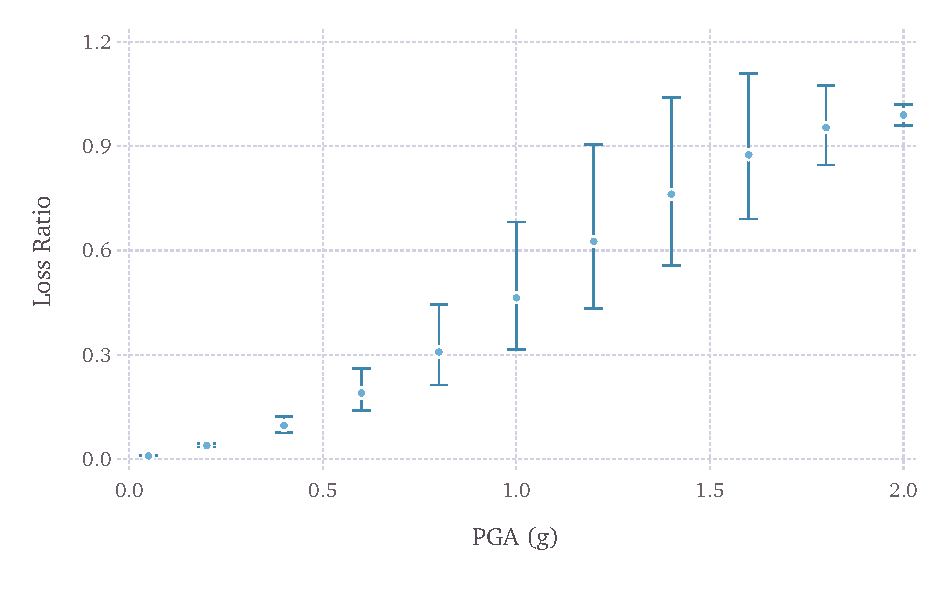
\includegraphics[width=12cm]{qareport/figures/fig-vf-ln-tax1-nzcov}
\caption{Vulnerability model with nonzero coefficients of variation}
\label{fig:vf-ln-tax1-nzcov}
\end{figure}

The vulnerability function for this case provides mean loss ratio values and coefficients of variation at intensity measure levels $PGA = 0.4 g$ and $0.6 g$, but none at $0.5 g$. Linear interpolation gives a mean loss ratio of $0.15$ for $PGA = 0.5 g$. Similarly, the coefficients of variation of the loss ratio at $0.4 g$ and $0.6 g$ are $0.24$ and $0.32$ respectively. The coefficient of variation of the loss ratio for $PGA = 0.5 g$ is obtained by linear interpolation as $0.28$.

The loss ratio at $PGA = 0.5 g$ follows a lognormal distribution with a mean of $0.15$ and a standard deviation of $0.28 \times 0.15 = 0.042$.

Since there is no variability in the ground motion, the expected value of the mean loss ratio for the scenario is also $0.15$, and the expected value of the standard deviation of the loss ratio is $0.042$.

These numbers are multiplied by the asset value of $10,000$ to give the expected mean and standard deviation of loss for the scenario as $1,500$ and $420$ respectively.
